\documentclass[aspectratio=169,10pt]{beamer}

% Compile on Overleaf with pdfLaTeX (run twice for the citations). No external files needed.
\usetheme{Madrid}
\usecolortheme{default}
\setbeamertemplate{navigation symbols}{}
\setbeamertemplate{footline}[frame number]
\usepackage[T1]{fontenc}
\usepackage[utf8]{inputenc}
\usepackage{lmodern}
\usepackage{booktabs}
\usepackage{array}
\usepackage{amsmath}
\usepackage{graphicx}
\usepackage{xcolor}
\usepackage{multicol}
\usepackage{multirow}
\usepackage{tikz}
\usetikzlibrary{positioning,arrows.meta}
\usepackage{pgfplots}
\pgfplotsset{compat=1.16}

\definecolor{MoABlue}{RGB}{25,70,115}
\definecolor{MoATeal}{RGB}{0,130,140}
\definecolor{MoALight}{RGB}{235,242,248}
\definecolor{MoAOrange}{RGB}{210,110,30}
\setbeamercolor{structure}{fg=MoABlue}
\setbeamercolor{frametitle}{bg=MoABlue,fg=white}
\setbeamercolor{title}{fg=white}
\setbeamercolor{block title}{bg=MoABlue,fg=white}
\setbeamercolor{block body}{bg=MoALight,fg=black}
\setbeamercolor{alerted text}{fg=MoATeal}

\title[MoA Prediction]{Mechanisms of Action Prediction}
\subtitle{A Multi-Model Ensemble for Highly Imbalanced Multi-Label Classification}
\author{Marco Merlonghi}
\institute{Project Work in Machine Learning and Data Mining}
\date{}

\newcommand{\metric}[1]{\textcolor{MoATeal}{\textbf{#1}}}
\newcommand{\smallnote}[1]{{\tiny\textit{#1}}}

\begin{document}

% 1
\begin{frame}
  \titlepage
  \vspace{-0.5em}
  \begin{center}
    \small Kaggle LISH MoA Prediction Challenge~\cite{moa}
  \end{center}
\end{frame}

% 2
\begin{frame}{The Problem}
\begin{block}{Prediction task}
Given the gene-expression and cell-viability profile of human cells exposed to a compound, predict which of 206 mechanisms of action (MoAs) the compound triggers.
\end{block}
\begin{itemize}
  \item \textbf{Multi-label}: a sample can have no positive label, one, or several.
  \item \textbf{Metric}: mean binary log loss over all samples and targets (lower is better).
  \item \textbf{Difficulty}: very sparse positives, strong target imbalance, and \emph{repeated measurements of the same compound}.
\end{itemize}
\begin{alertblock}{Central methodological question}
Does the validation score estimate generalisation to compounds that were not seen in training?
\end{alertblock}
\vspace{0.2em}
\textbf{Project objectives}
\begin{itemize}
  \item Reproducible cross-validated pipeline; compare neural and tree models; seed bagging.
  \item Compound-aware validation, and a measure of how optimistic row-wise CV is.
  \item Tuning that never selects on the scored fold; ensemble re-validated by nested CV.
\end{itemize}
\end{frame}

% 3
\begin{frame}{Data and Label Structure}
\begin{columns}[T,onlytextwidth]
\column{0.48\textwidth}
\begin{block}{Training set}
\begin{itemize}
  \item 23,814 rows: 21,948 treated and 1,866 control (7.8\%).
  \item 772 gene-expression (\texttt{g-*}) and 100 cell-viability (\texttt{c-*}) features.
  \item \texttt{cp\_time} (24/48/72 h), \texttt{cp\_dose} (D1/D2).
  \item 3,288 distinct compounds among treated rows (median 6 rows, maximum 718), from \texttt{train\_drug.csv}.
\end{itemize}
\end{block}
\column{0.48\textwidth}
\begin{block}{Labels}
\begin{itemize}
  \item Positive rate: \metric{0.373\%} of treated-row/target cells.
  \item 34.2\% of treated rows have no label, 57.1\% one, 8.7\% two or more.
  \item Positives per target: 1--832 (median 38); 53 targets have fewer than 20.
\end{itemize}
\end{block}
\end{columns}
\vspace{0.4em}
\begin{itemize}
  \item Controls have no MoA by definition: excluded from training, predicted as all zeros at inference.
  \item The test set has \textbf{no compound identifier}: overlap with training can only be inferred indirectly.
\end{itemize}
\end{frame}

% 4
\begin{frame}{Runs and Notation}
\small
Results refer to three training runs (all with the same code structure, 5 folds, 3-seed bagging):
\vspace{0.3em}

\begin{tabular}{llllc}
\toprule
\textbf{Run} & \textbf{CV protocol} & \textbf{Hyperparameters} & \textbf{Kaggle} & \textbf{Time (2$\times$T4)}\\
\midrule
R  & row-wise & defaults & yes & $\approx$130 min\\
H1 & hybrid (compound-aware) & tuning v2 (row-wise folds) & no & 75 min\\
H2 & hybrid (compound-aware) & tuning v3 (compound-aware folds) & yes & 95 min\\
\bottomrule
\end{tabular}
\vspace{0.5em}
\begin{itemize}
  \item H0: an earlier hybrid run (nested blend 0.01720), used only in the fold and compound diagnostics.
  \item \textbf{Deliverables} (Python notebooks): training, inference, three tuning versions, fold diagnostics, offline blend, test-overlap analysis, nearest-neighbour override test.
  \item Training and inference are separate: the training notebook saves the artifacts, the inference notebook writes \texttt{submission.csv} without retraining.
\end{itemize}
\smallnote{R used an earlier code revision; this matters for the interpretation of the R versus H comparison (slide 13).}
\end{frame}

% 5
\begin{frame}{End-to-End Pipeline}
\centering
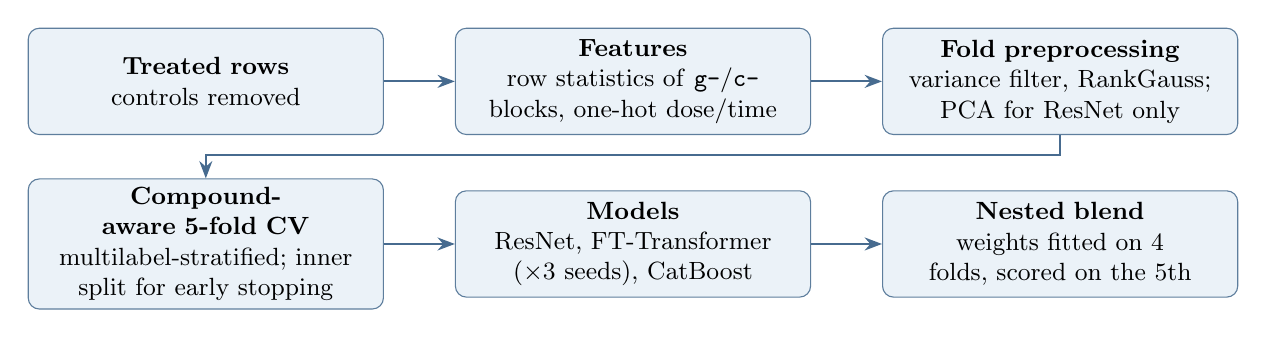
\begin{tikzpicture}[
    node distance=0.55cm and 0.9cm,
    block/.style={rectangle, rounded corners, draw=MoABlue!70, fill=MoALight, text width=4.3cm,
                  align=center, minimum height=1.35cm, inner sep=3pt, font=\small},
    arrow/.style={-{Stealth[length=2.2mm]}, thick, MoABlue!80}
]
\node[block] (data) {\textbf{Treated rows}\\ controls removed};
\node[block, right=of data] (feat) {\textbf{Features}\\ row statistics of \texttt{g-}/\texttt{c-} blocks, one-hot dose/time};
\node[block, right=of feat] (prep) {\textbf{Fold preprocessing}\\ variance filter, RankGauss;\\ PCA for ResNet only};
\node[block, below=of data] (cv) {\textbf{Compound-aware 5-fold CV}\\ multilabel-stratified; inner split for early stopping};
\node[block, right=of cv] (models) {\textbf{Models}\\ ResNet, FT-Transformer ($\times$3 seeds), CatBoost};
\node[block, right=of models] (blend) {\textbf{Nested blend}\\ weights fitted on 4 folds, scored on the 5th};
\draw[arrow] (data) -- (feat);
\draw[arrow] (feat) -- (prep);
\draw[arrow] (prep.south) -- ++(0,-0.25) -| (cv.north);
\draw[arrow] (cv) -- (models);
\draw[arrow] (models) -- (blend);
\end{tikzpicture}

\vspace{0.5em}
{\small Inference: fold pipelines and checkpoints are loaded, predictions averaged over folds and seeds, blended with the nested-CV weights; control rows set to 0.}
\end{frame}

% 6
\begin{frame}{Models and Preprocessing}
\small
\begin{columns}[T,onlytextwidth]
\column{0.31\textwidth}
\begin{block}{TabularResNet}
\begin{itemize}
  \item Residual MLP with batch norm and dropout.
  \item RankGauss $\rightarrow$ PCA (50 gene and 15 viability components) concatenated to the features.
\end{itemize}
\end{block}
\column{0.31\textwidth}
\begin{block}{FT-Transformer~\cite{ft}}
\begin{itemize}
  \item One token per feature, [CLS] token, self-attention.
  \item Simplified variant (post-LayerNorm, GELU).
  \item RankGauss only, no PCA.
\end{itemize}
\end{block}
\column{0.31\textwidth}
\begin{block}{CatBoost~\cite{cat}}
\begin{itemize}
  \item \texttt{MultiLogloss}, 250 iterations, one model per fold.
  \item RankGauss only, no PCA.
  \item Targets with no training positive: smoothed Jeffreys prior.
\end{itemize}
\end{block}
\end{columns}
\vspace{0.4em}
\textbf{Shared training choices}
\begin{itemize}
  \item \texttt{BCEWithLogitsLoss} with label smoothing 0.001~\cite{ls}; AdamW~\cite{adamw}; \texttt{ReduceLROnPlateau}; mixed precision~\cite{amp}.
  \item Early stopping (patience 8, at most 35 epochs) on an inner 10\% split built with the \emph{same grouping rule} as the outer folds; the outer fold is scored once.
  \item Fold-wise transforms (variance filter, RankGauss, PCA) are fitted on the training fold only~\cite{sklearn}.
\end{itemize}
\end{frame}

% 7
\begin{frame}{Cross-Validation Protocols}
\small
All protocols: 5-fold iterative multilabel stratification~\cite{strat,itstrat} on treated rows; the compound id comes from \texttt{train\_drug.csv}.
\vspace{0.3em}

\begin{tabular}{p{0.13\textwidth} p{0.2\textwidth} p{0.5\textwidth}}
\toprule
\textbf{Protocol} & \textbf{Unit kept together} & \textbf{Main property}\\
\midrule
\texttt{row} & single row & 99.4\% of validation rows have their compound in the training fold.\\
\texttt{grouped} & whole compound & No overlap, but compounds have up to 718 rows: fold sizes deviate up to 25.6\%.\\
\texttt{hybrid} & compound, except those with $>18$ rows (split by row) & 9 compounds (9.8\% of rows) split by row; fold sizes within 1.4\%; 9.8\% of validation rows share their compound with training.\\
\bottomrule
\end{tabular}
\vspace{0.4em}
\begin{block}{Why hybrid?}
Pure grouping is unbalanced and pessimistic for targets dominated by a few very large compounds; hybrid trades compound separation for balanced folds. The threshold is a \emph{design choice}, not a proven optimum.
\end{block}
\end{frame}

% 8
\begin{frame}{Choosing the Hybrid Threshold}
\small
Simulation on the real labels (one splitter seed): compounds with \emph{more} rows than the threshold are split by row.
\vspace{0.3em}

\centering
\begin{tabular}{lccc}
\toprule
\textbf{Scheme} & \textbf{Rows split by row} & \textbf{Max fold-size dev.} & \textbf{Val. rows with seen compound}\\
\midrule
pure grouped & 0\% & 25.6\% & 0\%\\
hybrid, $>6$ rows & 22.0\% & 3.4\% & 22.0\%\\
hybrid, $>12$ rows & 11.9\% & 3.1\% & 11.9\%\\
\textbf{hybrid, $>18$ rows} & \textbf{9.8\%} & \textbf{1.4\%} & \textbf{9.8\%}\\
hybrid, $>30$, $60$ or $100$ rows & 9.7\% & 2.8\% & 9.7\%\\
\bottomrule
\end{tabular}

\vspace{0.5em}
\raggedright
\begin{itemize}
  \item The rule: the \emph{largest} threshold that brings fold sizes within a few percent keeps as much of the compound-aware protocol as possible.
  \item Thresholds 30, 60 and 100 give identical splits (8 compounds); the difference between 1.4\% and 2.8\% is within what another seed could change.
  \item The sensitivity of the CV \emph{loss} to the threshold was not measured.
\end{itemize}
\end{frame}

% 9
\begin{frame}{Ensemble and Nested Blending}
\begin{itemize}
  \item Predictions averaged over 3 seeds (and folds) for each network; CatBoost: one model per fold.
  \item Weights on the simplex via softmax reparameterisation, optimised with Nelder--Mead~\cite{nm} on out-of-fold predictions.
  \item \textbf{Nested estimate}: weights fitted on four folds, score measured on the fifth, rotating the held-out fold.
\end{itemize}
\[
\hat{p}_{\mathrm{ens}} = w_R\hat{p}_{R} + w_F\hat{p}_{F} + w_C\hat{p}_{C},
\qquad w_R+w_F+w_C=1
\]
\begin{columns}[T,onlytextwidth]
\column{0.5\textwidth}
\begin{block}{Final weights (ResNet / FT / CatBoost)}
\small
R: 0.453 / 0.375 / 0.173\\
H1: 0.371 / 0.405 / 0.225\\
H2: 0.478 / 0.348 / 0.175
\end{block}
\column{0.46\textwidth}
\begin{block}{Optimism of the blending step}
\small
In-sample minus nested score: $1.6\cdot10^{-6}$ (R), $2.8\cdot10^{-6}$ (H1), $2.6\cdot10^{-6}$ (H2): negligible with three weights.
\end{block}
\end{columns}
\vspace{0.3em}
\smallnote{The nested estimate limits optimism from fitting the weights; it does not remove bias from the CV design or from model selection.}
\end{frame}

% 10
\begin{frame}{Hyperparameter Tuning: Three Versions}
\small
Optuna~\cite{optuna} with TPE sampler~\cite{tpe} and median pruner; the default configuration is trial 0 of every study (v2, v3).
\vspace{0.3em}

\begin{tabular}{p{0.07\textwidth} p{0.2\textwidth} p{0.3\textwidth} p{0.3\textwidth}}
\toprule
 & \textbf{Folds} & \textbf{Model selection in a trial} & \textbf{Adoption rule}\\
\midrule
v1 & 5 row-wise & best epoch on the \emph{scored} fold (flawed, not used by any reported run) & lowest mean loss\\
v2 & fold 0 search, fold 1 confirm (row-wise) & 10\% inner split & better than default on both folds, gain $\ge 5\cdot10^{-5}$\\
v3 & as v2, compound-aware, own split seed & 10\% compound-aware inner split & gain $\ge 10^{-4}$ on the confirmation fold \emph{and} wins on more than half of 3 paired seeds\\
\bottomrule
\end{tabular}
\vspace{0.4em}
\begin{itemize}
  \item v3 decides only on the confirmation fold: the search-fold score is the minimum over $N$ trials, hence biased.
  \item Search: 25/15/15 trials for ResNet/FT/CatBoost, one seed per trial.
  \item v3 found no FT-Transformer candidate better than the default: it keeps default values.
\end{itemize}
\end{frame}

% 11
\begin{frame}{Selected Hyperparameters}
\scriptsize
\centering

\setlength{\tabcolsep}{6pt}
\renewcommand{\arraystretch}{1.2}

\begin{tabular}{llccc}
\toprule
\textbf{Model} & \textbf{Parameter} & \textbf{Default} & \textbf{H1 (v2)} & \textbf{H2 (v3)}\\
\midrule

\multirow{4}{*}{ResNet}
 & Learning rate & $10^{-3}$ & $1.18\cdot10^{-3}$ & $2.67\cdot10^{-3}$\\
 & Dropout & 0.2 & 0.427 & 0.583\\
 & Weight decay & $10^{-5}$ & $8.5\cdot10^{-6}$ & $2.66\cdot10^{-4}$\\
 & Hidden units / batch & 512 / 256 & 768 / 128 & 768 / 512\\

\midrule
FT-Transformer
 & LR / dropout / WD & $10^{-3}$ / 0.2 / $10^{-5}$ & $2.35\cdot10^{-3}$ / 0.063 / $9.9\cdot10^{-6}$ & Default\\

\midrule
\multirow{2}{*}{CatBoost}
 & Depth / L2 & 5 / 3 & 4 / 19.0 & 4 / 56.0\\
 & LR / subsample & 0.08 / -- & 0.1034 / 0.829 & 0.1034 / 0.829\\

\bottomrule
\end{tabular}

\vspace{0.6em}
\raggedright
\small
\begin{itemize}
  \item In v3, ResNet dropout (0.583), batch size (512) and learning rate ($2.67\cdot10^{-3}$) lie at or near the search-space bounds.\\ The optimum may be outside the search space.
  \item CatBoost learning rate and subsample coincide in H1 and H2 (same seeded sampler draw); OOF does not change (0.01782 vs 0.01783).
\end{itemize}
\end{frame}

% 12
\begin{frame}{Results: Cross-Validation}
\small
Out-of-fold log loss on treated rows (lower is better); networks use seed-averaged predictions.
\vspace{0.2em}

\centering
\begin{tabular}{lccc}
\toprule
\textbf{Model} & \textbf{R: row/default} & \textbf{H1: hybrid/v2} & \textbf{H2: hybrid/v3}\\
\midrule
Baseline (per-target prior) & 0.02220 & 0.02233 & 0.02233\\
TabularResNet & 0.01632 & 0.01744 & 0.01735\\
FT-Transformer & 0.01643 & 0.01736 & 0.01744\\
CatBoost & 0.01699 & 0.01782 & 0.01783\\
\midrule
\textbf{Nested ensemble} & \textbf{0.01607 $\pm$ 0.00017} & \textbf{0.01714 $\pm$ 0.00031} & \textbf{0.01715 $\pm$ 0.00031}\\
\bottomrule
\end{tabular}
\vspace{0.4em}

\raggedright
\begin{itemize}
  \item Ensemble improves on the best single model by about 1.5\% (R) and 1.2\% (H2).
  \item \textbf{Each model contributes} (H2, drop-one nested blend): without ResNet $+1.2\cdot10^{-4}$, without FT $+0.8\cdot10^{-4}$, without CatBoost $+0.6\cdot10^{-4}$; removing any one worsens the score in all five folds.
  \item Residual correlations are high (0.98 between networks); CatBoost is the most different on positive cells (0.945).
\end{itemize}
\end{frame}

% 13
\begin{frame}{Row-Wise versus Compound-Aware CV}
\small
\begin{alertblock}{Not a controlled comparison}
The $+6.7\%$ from R (0.01607) to H2 (0.01715) also reflects code revision, hyperparameters and fold assignment.
\end{alertblock}
\vspace{0.2em}
Paired decomposition (blend; run H0 against the row-wise OOF, same rows), bootstrap over compounds:
\vspace{0.2em}

\centering
\begin{tabular}{lcccc}
\toprule
\textbf{Rows} & \textbf{Share} & \textbf{Loss row-wise} & \textbf{Loss hybrid} & \textbf{Contribution to gap}\\
\midrule
Frequent compounds & 9.8\% & 0.00172 & 0.00198 & $+0.00003$\\
All other rows & 90.2\% & 0.01762 & 0.01885 & $+0.00111$\\
\bottomrule
\end{tabular}

\vspace{0.4em}
\raggedright
\begin{itemize}
  \item On ordinary compounds: $+0.00123$ per row ($+7.0\%$), 95\% interval over compounds $[+0.00112,+0.00135]$.
  \item Almost the whole difference sits on rows that hybrid CV evaluates as \emph{unseen}.
  \item The worst hybrid fold (fold 4, $+4.7\%$) is \emph{not} explained by frequent compounds: fold spread 0.00091 on all rows, 0.00095 without them.
  \item Labels are identical across all rows of each of the 8 largest compounds; e.g.\ 98.9\% of \texttt{proteasome\_inhibitor} positives come from one compound.
\end{itemize}
\end{frame}

% 14
\begin{frame}{Per-Target Analysis (H2 blend)}
\begin{columns}[T,onlytextwidth]
\column{0.52\textwidth}
\small
\textbf{Skill} $=1-\text{loss}/\text{loss of the per-target prior}$, by number of positives (row-wise vs hybrid):
\vspace{0.3em}

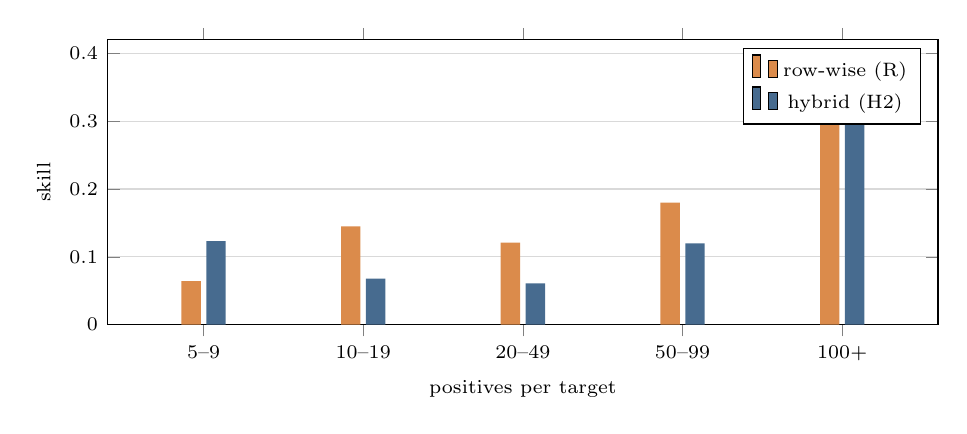
\begin{tikzpicture}
\begin{axis}[
  ybar, width=\textwidth, height=5.2cm, bar width=7pt,
  ymin=0, ymax=0.42, ylabel={skill}, ylabel style={font=\scriptsize},
  xtick={1,2,3,4,5}, xticklabels={5--9,10--19,20--49,50--99,100+},
  xlabel={positives per target}, xlabel style={font=\scriptsize},
  tick label style={font=\scriptsize}, enlarge x limits=0.15,
  legend style={font=\scriptsize, at={(0.98,0.97)}, anchor=north east},
  ymajorgrids, grid style={gray!30}
]
\addplot[fill=MoAOrange!80, draw=none] coordinates {(1,0.064) (2,0.145) (3,0.121) (4,0.180) (5,0.374)};
\addplot[fill=MoABlue!80, draw=none] coordinates {(1,0.123) (2,0.068) (3,0.061) (4,0.120) (5,0.342)};
\legend{row-wise (R), hybrid (H2)}
\end{axis}
\end{tikzpicture}

\smallnote{The per-target baseline differs between protocols: skills are not strictly comparable. Bin 1--4 (2 targets) omitted.}
\column{0.45\textwidth}
\small
\begin{itemize}
  \item The 41 targets with $\ge100$ positives carry 47.9\% of the loss (skill 0.342).
  \item The 53 \emph{rare} targets ($<20$ positives) carry 6.6\% of the loss; skill $+0.080$ [0.056, 0.102]; for 8 of them the model does not beat the prior.
  \item The blend over-predicts rare targets: expected/observed positives 1.47 below 20 positives.
  \item 31 targets with $\ge10$ positives come from at most 3 compounds: close to compound-identity labels.
\end{itemize}
\end{columns}
\end{frame}

% 15
\begin{frame}{Independent Check: Kaggle Test Set}
\small
Two late submissions through the inference notebook (one per configuration).
\vspace{0.3em}

\centering
\begin{tabular}{lcc}
\toprule
 & \textbf{R} & \textbf{H2}\\
\midrule
Nested-CV blend, treated rows & 0.01607 & 0.01715\\
Rescaled to all test rows ($\times0.910$) & 0.01462 & 0.01561\\
Kaggle private & 0.01634 & 0.01643\\
Kaggle public & 0.01865 & 0.01873\\
Private above rescaled CV & $+11.8\%$ & $+5.3\%$\\
Public above rescaled CV & $+27.5\%$ & $+20.0\%$\\
\bottomrule
\end{tabular}
\vspace{0.4em}

\raggedright
\begin{itemize}
  \item Hybrid CV is closer to the private score and reproduces about 57\% of the gap between the row-wise estimate and the private score. This is indirect evidence, not a proof.
  \item The two submissions differ by $9\cdot10^{-5}$ (private) and $8\cdot10^{-5}$ (public): \textbf{they cannot be ranked}; protocol, tuning and model selection did not move the test score measurably.
  \item Public and private scores differ by 0.0023 for \emph{both}: the test subsets differ in difficulty.
\end{itemize}
\smallnote{The test set was never used to tune or select; it did motivate the compound-aware protocols. The rescaling uses the public treated share (0.910): approximate.}
\end{frame}

% 16
\begin{frame}{Do the Test Compounds Overlap with Training?}
\small
Indirect analysis from nearest-neighbour cosine distances (no compound id in the test set).
\begin{itemize}
  \item \textbf{General overlap: not assessable.} Distance separates seen from unseen compounds poorly (AUC 0.516); the mixture estimate must be discarded.
  \item \textbf{Frequent compounds} (5 of 8 analysed are present):
\end{itemize}
\vspace{0.2em}

\centering
\scriptsize
\begin{tabular}{lcccc}
\toprule
\textbf{Compound} & \textbf{Test rows assigned} & \textbf{Expected if absent} & \textbf{Test share} & \textbf{Train share}\\
\midrule
\texttt{87d714366} & 133 & 5.3 & 3.93\% & 3.27\%\\
\texttt{8b87a7a83} & 23 & 0.5 & 0.69\% & 0.92\%\\
\texttt{d1b47f29d} & 24 & 0.5 & 0.72\% & 0.81\%\\
\texttt{d08af5d4b} & 36 & 11.4 & 0.83\% & 0.89\%\\
\texttt{292ab2c28} & 18 & 6.2 & 0.38\% & 0.88\%\\
\bottomrule
\end{tabular}

\vspace{0.4em}
\raggedright\small
\begin{itemize}
  \item Four are at about their training frequency; \texttt{292ab2c28} at about half of it.
  \item For the other three the assigned rows are close to those expected if absent: presence cannot be established.
  \item A back-of-the-envelope reweighting with the hybrid losses gives an all-rows estimate of 0.0156--0.0161 against 0.01643 private (residual gap 2--5\%): inference, not measurement.
\end{itemize}
\end{frame}

% 17
\begin{frame}{Negative Results}
\small
\begin{columns}[T,onlytextwidth]
\column{0.5\textwidth}
\begin{block}{Nearest-neighbour override for frequent compounds}
\begin{itemize}
  \item Pull predictions of rows assigned to a frequent compound towards its label profile (parameters from the training part of each fold).
  \item Rule precision 0.722, recall 0.809; gain ceiling only $1.7\cdot10^{-4}$.
  \item All four variants \textbf{worsen} the OOF loss on all five folds: from $+2.1\cdot10^{-4}$ (mixture 0.5) to $+1.47\cdot10^{-3}$ (replacement).
  \item Cost sits on false assignments (663 of 2,381 rows).
\end{itemize}
\end{block}
\column{0.47\textwidth}
\begin{block}{Extra networks (run R protocol)}
\scriptsize
\begin{tabular}{lcc}
\toprule
\textbf{Configuration} & \textbf{Ensemble} & \textbf{Extra weight}\\
\midrule
+ MLP (PCA) & 0.01604 & 0.015\\
+ 1D-CNN (PCA) & 0.01605 & 0.082\\
+ 1D-CNN (raw) & 0.01606 & 0.070\\
no extra network & 0.01605--0.01606 & --\\
\bottomrule
\end{tabular}
\vspace{0.3em}
\small
Differences $\le 2\cdot10^{-5}$: below the fold standard deviation (0.00017) and comparable to run-to-run noise ($\approx10^{-5}$).
\end{block}
\end{columns}
\vspace{0.4em}
\begin{alertblock}{Takeaway}
More components or compound-specific post-processing gave no robust gain on the available validation evidence: the simpler three-model ensemble was kept.
\end{alertblock}
\end{frame}

% 18
\begin{frame}{Limitations}
\small
\begin{enumerate}
  \item \textbf{Test compound ids unknown:} overlap is inferred only for frequent compounds; ordinary-compound overlap is unassessed, so neither hybrid nor pure grouped CV can be declared the faithful one.
  \item \textbf{Hybrid threshold is heuristic:} 18 rows chosen from fold balance for one seed; CV-loss sensitivity not measured.
  \item \textbf{Non-controlled protocol comparison:} R and H runs differ in code, hyperparameters and folds.
  \item \textbf{Selection bias:} tuning and model choices reused folds overlapping the reported OOF; no untouched hold-out; nested selection of the whole procedure was too costly.
  \item \textbf{Limited tuning:} one seed per trial, few trials, optimum possibly outside the ResNet search space; no controlled tuned-vs-default comparison under hybrid CV.
  \item \textbf{Preprocessing:} unsupervised transforms include inner-validation rows; may slightly affect early stopping.
  \item \textbf{Test evidence:} two submissions, noisy and different public/private subsets; fold standard deviation (0.0003) understates the uncertainty on unseen data.
  \item \textbf{Reproducibility:} GPU non-determinism ($\approx10^{-5}$); inference needs the separately saved artifact dataset.
\end{enumerate}
\end{frame}

% 19
\begin{frame}{Conclusions}
\begin{itemize}
  \item A reproducible training/inference workflow for a sparse 206-target multi-label task, with separated notebooks and saved artifacts.
  \item Compound-aware CV exposes a harder generalisation setting than row-wise CV: the extra loss sits almost entirely on ordinary compounds that become ``unseen''.
  \item The three-model ensemble beats each component in the nested-CV experiments (each model helps in all five folds).
  \item Tuning did not measurably improve the hybrid ensemble; the two Kaggle submissions cannot be ranked against each other.
  \item Nearest-neighbour post-processing and extra networks brought no gain: simplicity was preferred.
\end{itemize}
\vspace{0.5em}
\begin{alertblock}{Main lesson}
For repeated-compound biological measurements, validation design can matter at least as much as model architecture. A CV score must be read together with the assumptions of its split, here the unknown overlap between test and training compounds.
\end{alertblock}
\end{frame}

% 20
\begin{frame}{References}
\footnotesize
\tiny
\begin{thebibliography}{99}
\bibitem{moa} Kaggle. \emph{Mechanisms of Action (MoA) Prediction}, 2020. \url{https://www.kaggle.com/competitions/lish-moa}
\bibitem{ft} Gorishniy, Y., Rubachev, I., Khrulkov, V., Babenko, A. \emph{Revisiting Deep Learning Models for Tabular Data}. NeurIPS, 2021.
\bibitem{cat} Prokhorenkova, L. et al. \emph{CatBoost: unbiased boosting with categorical features}. NeurIPS, 2018.
\bibitem{strat} Sechidis, K., Tsoumakas, G., Vlahavas, I. \emph{On the Stratification of Multi-Label Data}. ECML PKDD, 2011.
\bibitem{itstrat} Bradberry, T. \emph{iterative-stratification} (Python package). \url{https://github.com/trent-b/iterative-stratification}
\bibitem{adamw} Loshchilov, I., Hutter, F. \emph{Decoupled Weight Decay Regularization}. ICLR, 2019.
\bibitem{amp} Micikevicius, P. et al. \emph{Mixed Precision Training}. ICLR, 2018.
\bibitem{ls} Szegedy, C. et al. \emph{Rethinking the Inception Architecture for Computer Vision}. CVPR, 2016 (label smoothing).
\bibitem{optuna} Akiba, T. et al. \emph{Optuna: A Next-generation Hyperparameter Optimization Framework}. KDD, 2019.
\bibitem{tpe} Bergstra, J., Bardenet, R., Bengio, Y., K\'egl, B. \emph{Algorithms for Hyper-Parameter Optimization}. NeurIPS, 2011.
\bibitem{nm} Nelder, J.A., Mead, R. \emph{A simplex method for function minimization}. The Computer Journal 7(4), 1965.
\bibitem{sklearn} Pedregosa, F. et al. \emph{Scikit-learn: Machine Learning in Python}. JMLR 12, 2011.
\end{thebibliography}
\end{frame}

\end{document}